\documentclass[a4paper]{scrartcl}
\usepackage[utf8]{inputenc}			% Für Umlaute
\usepackage[T1]{fontenc}			% Für richtige Schrift
\usepackage[ngerman]{babel}			% Für neue deutsche Rechtschreibung (Trennung)
\usepackage{color}
\usepackage{amsmath}
\usepackage{amssymb}
\usepackage{graphicx}
\usepackage{textcomp}				% Fürs Gardzeichen

\usepackage{scrpage2}				% Für Kopf- und Fußzeilen
\pagestyle{scrheadings}				% Für Kopf- und Fußzeilen
\clearscrheadfoot					% Für Kopf- und Fußzeilen

\renewcommand{\labelenumi}{\alph{enumi})}
\renewcommand{\labelenumii}{\alph{enumii})}

\begin{document}
\titlehead{Wintersemester 2017/2018\\Motion Planning\\Prof. Horsch, Rudi Scheitler}
\author{David Welsch, Ken Hasenbank}
\title{Praktikum 3 - Visibility Graph}
\maketitle

\section*{Beschreibung der Aufgabe}

In diesem Praktikum sollte die Wegfindung mit Hilfe des Visibility-Graphs realisiert werden.
\\\\
Ein Visibility-Graph beinhaltet Punkte aus einem Konfigurationsraum sowie die Kanten zwischen diesen Punkten, welche kollisionsfrei verbunden werden können. Der Name \textit{Visibility}-Graph kommt zu Stande, da die Kanten auch als Sichtverbindungen zwischen den Punkten gedeutet werden können. Ein Beispiel für einen Visibility-Graph ist in Abbildung \ref{img:GraphBsp} zu sehen.\\
\begin{figure}[h!]
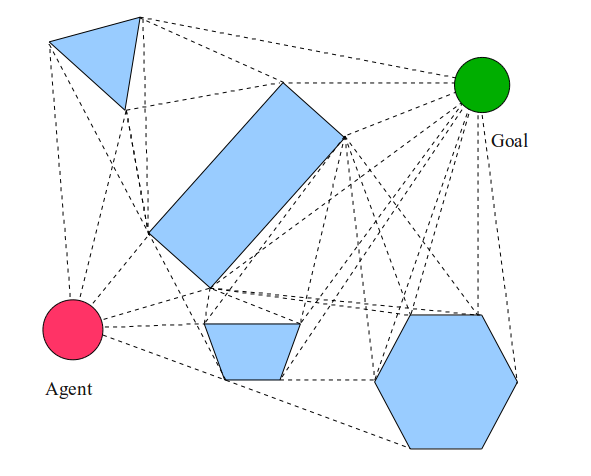
\includegraphics[width=\textwidth]{graph1.png}
\caption{Visibility Graph}
\label{img:GraphBsp}
\end{figure}
\begin{figure}[h!]
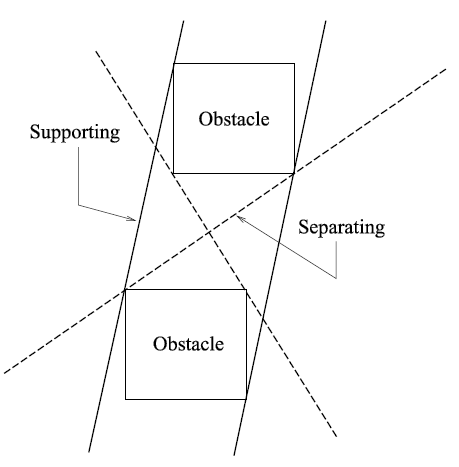
\includegraphics[width=\textwidth]{Reduced.PNG}
\caption{Reduced Visibility Graph}
\label{img:RedGraph}
\end{figure}
Bei diesem Graph kann man sehen, dass die Verbindungen entlang der Sichtlinien, jeweils von den Ecken der Hindernisse zu Ecken andere Hindernisse, bzw. vom und zum Start-/Zielpunkt, gezeichnet sind. In der Abbildung wird der Startpunkt als \textit{Agent} bezeichnet, der Zielpunkt als \textit{Goal}.\\

In diesem Praktikum soll nun zuerst ein Visibility-Graph erstellt werden. Im nächsten Schritt muss dann auf diesem Graphen mit Hilfe eines Wegfindungs-Algorithmus, zum Beispiel Dijkstra oder der A\* -Algorithmus, der kürzeste Pfad von Start zu Zielpunkt gefunden werden.\\

Beim freiwilligen Teil der Aufgabe haben wir uns darauf geeinigt, einen auf \textit{Supporting}- und \textit{Separating}-Lines reduzierten Visibility-Graphen zu erstellen. Ein solcher reduzierten Graph ist in Abbildung \ref{img:RedGraph} zu sehen.

\section*{Beschreibung der L"osung}

Im Anhang sind die von Gnuplot erstellten Plots der einzelnen Graphen zu sehen.\\

Zur L"osung haben wir den vorgegeben Code-Rahmen, jedoch auf Grund verschiedener Probleme auf unseren Entwicklungsrechnern nicht die gesamte Boost-Library, verwendet. Zur Lösung haben wir ebenfalls die Klasse \textit{Linie} neu geschrieben, welche viele Hilfsfunktionen enthält. Die eigentliche Lösung wird mit Hilfe dieser Hilfsfunktionen in der Funktion und Klasse \textit{VisibilityGraph} berechnet. Anhand dieser Funktion beschriebe ich nun unser Vorgehen.

\begin{itemize}
	\item (Zeile 26) Zuerst wird ein Vektor erstellt, welcher später die Punkte auf dem kürzesten Pfad enthält.
	\item (35-38) Dann werden vier Graphen erstellt. Diese enthalten später die folgenden Kanten. Initial werden alle mit den Kanten aus dem Graph \textit{g} befüllt.
	\begin{itemize}
		\item obstacleGraph: Wird mit den Außenkanten der Hindernisse befüllt
		\item illegalLinesGraph: Wird mit den diagonalen Verbindungslinien der Hindernisse befüllt
		\item visibilityGraph: Dieser Graph wird nachher den berechneten Visibility-Graph beinhalten
		\item pathGraph: Dieser Graph wird am Ende den als am Kürzesten berechneten Pfad enthalten
	\end{itemize}
	Zusätzlich wird noch ein Vektor aus Obstacles erstellt, welcher die selbst erstellte Struktur Obstacle enthält. Diese Struktur wird später näher beschrieben.
	\item (Zeile 42) Im nächsten Schritt wird in der Variable \textit{knoten} die Anzahl der im Graphen \textit{g} enthaltenen Eckpunkte gespeichert.
	\item (Zeile 45-51) Dann wird eine Adjazenzliste in Form eines zwei-dimensionalen double-Arrays erstellt und mit der Gewichtung $-1$ initialisiert. $-1$ bedeutet, dass die Punkte nicht verbunden sind. Ansonsten enthält diese Liste die Länge der Kante zwischen den Punkten.
	\item (Zeile 53-54) Hier werden zwei Vektoren aus der selbst erstellten Klasse \textit{Linie} erstellt, welche mit den Kanten der Hindernisse (\textit{obstLines}) bzw. den Kanten innerhalb der Hindernisse (\textit{illegalLines}) befüllt werden soll.
	\item (Zeiel 55-81) In dieser for-Schleife werden die zuvor erstellten Vektoren mit den Diagonalen im Hindernis bzw. den Hinderniswänden befüllt. Um dies zu realisieren wird in der äußeren Schleife über alle Hindernisse iteriert. Bei jedem Schleifendurchlauf wird zusätzlich jeweils ein mal über die beiden gegenüberliegenden Punkte (Zeile 59-67), sowie über alle Punkte (Zeile 70-79) des jeweiligen Hindernissen iteriert.\\
	In der ersten Schleife werden die Diagonalen erstellt, in der zweiten die Kanten der Hindernisse.
	\item (Zeile 84-114) In dieser for-Schleife wird der eigentliche Visibility-Graph erstellt sowie die Adjazenzliste mit den richtigen Werten für die Gewichtung gefüllt. Dies geschieht wie folgt:\\
	\begin{itemize}
		\item (Zeile 84) Es wird über alle in dem Graph \textit{g} enthaltenen Punkte iteriert.
		\item (Zeile 85) Für jeden untersuchten Punkt wird erneut durch alle Punkte gelaufen, jedoch diesmal startend vom aktuell untersuchten Knoten, damit keine Verbindungen doppelt untersucht werden.
		\item (Zeile 86-88) Die Punkte am Index \textit{i} und \textit{j}, sowie die Linie zwischen diesen beiden Punkten wird zwischengespeichert.
		\item (Zeile 91) Anhand der Hilfsfunktionen \textit{isIllegal} und \textit{isVisible} (werden später erklärt) wird überprüft, ob die eben zwischengespeicherte Linie eine der Diagonalen in den Hindernissen ist (\textit{isIllegal}) und ob sie eine Außenkante der Hindernisse schneidet (\textit{isVisible}).
		\item (Zeile 108) Ist die Linie keine Diagonale der Hindernisse und schneidet sie keine der Kanten der Hindernisse wird sie zum \textit{visibilityGraph} hinzugefügt.
		\item (Zeile 109-110) In der Adjazenzmatrix wird zusätzlich die Länge der Linie in beide Richtungen gespeichert.
		
	\end{itemize}
	\item (Zeile 115) Die Adjazenzmatrix wird zu Debugzwecken auf der Console ausgegeben.
	\item (Zeile 117) Es wird ein Vektor des Typs \textit{int} erstellt, welcher durch die Funktion dijkstra mit Zahlen befüllt wird. Dieser Vektor enthält dann die Nummern der Knoten, welche den kürzesten Weg darstellen.\\
	Die Funktion \textit{dijkstra} enthält den Code des Dijkstra-Algorithmus und berechnet mit Hilfe dessen die entsprechenden Weg-Knoten.
	\item (Zeile 119-133) Anschließend werden die Kantennummern auf der Konsole ausgegeben und die Kanten des Weges in den Graphen \textit{pathGraph} gespeichert. In den Zeilen 129 und 130 werden die Punkte aus dem ursprünglichen Graphen \textit{g} in den Vektor \textit{path} gespeichert. Dieser repräsentiert dann den Weg.
	\item (Zeile 140-143) Hier werden die Graphen erstellt, damit sie mit GnuPlot visualisiert werden können.
\end{itemize}

Die so berechnete Lösung ist in Abbildung \ref{img:Lsg} im Anhang ersichtlich.

\subsection*{Beschreibung der Hilfsklasse \textit{Linie}}
Die Hilfsklasse \textit{Linie} enthält alle nötigen Funktionen um die oben beschriebene Lösung zu berechnen. Ich werde nacheinander alle Funktionen beschreiben.

\begin{itemize}
\item orientierungZurLinie(Point test)\\
Mit dieser Funktion wird die Orientierung eines Punktes zu der Linie berechnet und als Integer codiert zurückgegeben. Die Rückgabewerte haben folgende Bedeutung:\\
0 = Der Punkt befindet sich auf der Linie\\
1 = Der Punkt befindet sich rechts von der Linie\\
2 = Der Punkt befindet sich links von der Linie\\
\item schneidetLinie(Linie test)\\
Mit dieser Funktion wird berechnet, ob eine andere Linie diese Linie schneidet. Hierfür wird zuerst mit Hilfe der Funktionen \textit{compare} und \textit{extends} gestet, ob die Linien oder Start bzw. Endpunkte identisch sind. Anschließend werden die Orientierungen der Start- und Endpunkte der beiden Linien mit Hilfe der Funktion \textit{orientierungZurLinie} miteinander verglichen. Sind die Orientierung der Anfangs- und Endpunkte jeweils unterschiedlich, so schneiden sich die Linien und es wird true zurückgegeben. Ansonsten wird false zurückgegeben da sie sich nicht schneiden.
\item compare(Linie test)\\
In dieser Funktion wird verglichen ob die Linien identisch sind. Hierbei spielt die Orientierung keine Rolle.
\item extends(Linie test)\\
Diese Funktion berechnet, ob die Linien in einem Anfangs- oder Endpunkt identisch sind. 
\item getObstOrientierung(Obstacle obst)\\
Hier wird berechnet, wie ein Obstacle zu der Linie liegt. Ein Obstacle ist beschrieben durch das struct \textit{Obstacle}, welches aus einem Vektor aus Linien besteht. Die Funktion gibt zurück, ob die Linie durch das Obstacle geht, rechts, oder links davon liegt. Die Kodierung entspricht der von \textit{orientierungZurLinie}.
\item isSeparating(Obstacle obst1, Obstacle obst2)\\
Diese Funktion berechnet anhand zweier Obstacles, ob die Linie durch eines der beiden Obstacles hindurch verläuft und die beiden Obstacles auf derselben Seite der Linie liegen. Treffen alle drei Bedingungen nicht zu, wird false zurückgegeben. Das bedeutet, dass die Linie in Bezug auf die beiden übergebenen Obstacles keine Seperating-Line ist.
\item isSupporting(Obstacle obst1, Obstacle obst2)\\
Hie wird berechnet, ob die Linie eine Supporting-Line ist. Hierfür werden diesselben Dinge berechnet wie in der vorherigen Funktion, jedoch werden sie anders ausgewertet:\\
Die Linie darf nicht durch eines der Obstacles verlaufen, jedoch müssen beide Obstacles auf derselben Seite des Objektes sein. Dann ist die Linie eine Supporting-Line.\\
\item length()\\
Berechnet die Länge der Linie.
\end{itemize}


\subsection*{Beschreibung der Zusatzaufgabe (Reduzierter Visibility Graph)}
Die Zusatzaufgabe wird in der Datei \textit{VisibilityGraph.cpp} in den Zeilen 94 bis 106 gelöst. Dies geschieht wie folgt:\\
In jeder zuvor als mögliche Verbindung gefundenen Linie wird mit Hilfe der Funktionen \textit{isSupporting} und \textit{isSeparating} aus der Klasse \textit{Linie} geprüft, ob es sich bei der gerade geprüften Linie um eine solche handelt. Nur wenn eine der beiden Funktionen \textit{true} zurück gibt, wird die Linie auch in den \textit{visibilityGraph} aufgenommen, ansonsten wird durch \textit{continue} die nächste Linie überprüft.\\
Die vorher im Vektor \textit{obstacles} gespeicherten Hindernisse werden hierfür genutzt.\\

Die Lösung ist in Abbildung \ref{img:LsgZusatz} zu sehen.

\section*{Was wir gelernt haben}

Die Erstellung des Visibility Graphs war eine große Herausforderung. Zusätzlich hatten wir große Probleme mit der Boost-Library, da benötigte imports nicht funktioniert haben. Wir haben uns deshalb entschlossen, die entsprechenden Funktionen selbst zu implementieren und hatten damit schneller Erfolg.\\
Die Zusatzaufgabe stellte noch mal eine Herausforderung dar, aber nach reichlicher Überlegung konnten wir auch diese erfolgreich lösen.\\
Insgesamt war diese Praktikumsaufgabe sehr aufschlussreich und interessant.
\newpage
\section*{Anhang}

\begin{figure}[h!]
	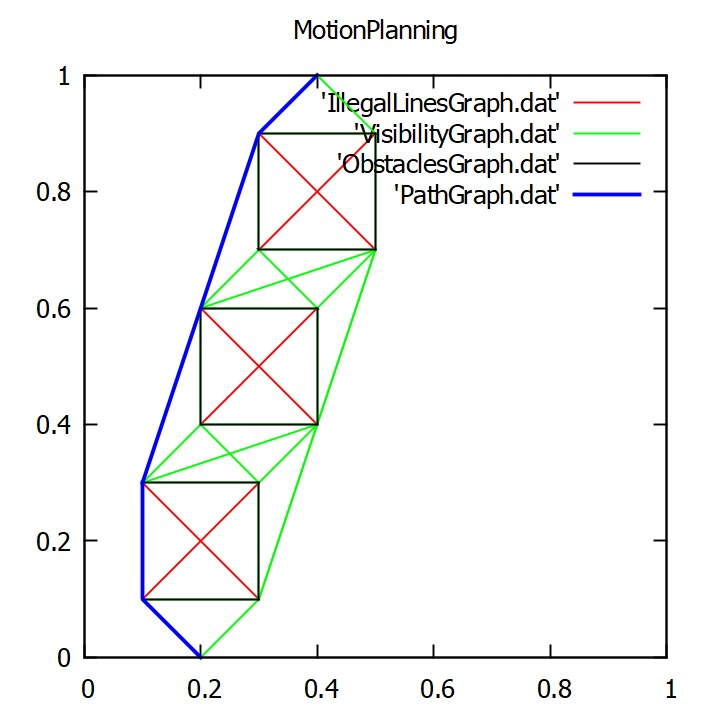
\includegraphics[height=0.4\textheight]{Visgraph.jpg}
	\caption{Lösung - ohne Zusatzaufgabe}
	\label{img:Lsg}
\end{figure}
\begin{figure}[h!]
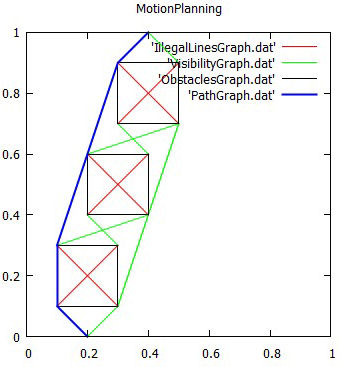
\includegraphics[height=0.4\textheight]{Visgraph_reduced.jpg}
\caption{Lösung - mit Zusatzaufgabe}
\label{img:LsgZusatz}
\end{figure}


\end{document}